\documentclass[tikz,border=3pt]{standalone}
\usepackage{fontspec}
\IfFontExistsTF{Times New Roman}
  {\setmainfont{Times New Roman}}
  {\setmainfont{TeX Gyre Termes}}
\usepackage{amsmath,amssymb}
\usepackage{xcolor}
\usepackage{tikz}
\usetikzlibrary{arrows.meta,positioning,calc,fit,backgrounds,shapes.geometric,decorations.pathreplacing,pgfplots.groupplots}
\definecolor{QFlowNavy}{HTML}{17365D}
\definecolor{QFlowBlue}{HTML}{2F5597}
\definecolor{QFlowTeal}{HTML}{2A7F7F}
\definecolor{QFlowAmber}{HTML}{8B5A00}
\definecolor{QFlowGray}{HTML}{667085}
\definecolor{QFlowLine}{HTML}{CBD5E1}
\definecolor{QFlowPaleBlue}{HTML}{EAF1F8}
\definecolor{QFlowPaleGray}{HTML}{F2F4F7}
\tikzset{
  qbox/.style={draw=QFlowNavy,rounded corners=1.2mm,fill=white,
    line width=0.6pt,align=center,inner sep=2.2mm,font=\fontsize{8.5}{10}\selectfont},
  qsoft/.style={qbox,fill=QFlowPaleBlue},
  qoutside/.style={qbox,draw=QFlowGray,dashed,fill=QFlowPaleGray},
  qarrow/.style={-{Latex[length=2mm,width=1.3mm]},line width=0.7pt,QFlowNavy},
  qdasharrow/.style={qarrow,dashed,QFlowGray},
  qlabel/.style={font=\fontsize{8}{9.2}\selectfont,align=center},
  qsmall/.style={font=\fontsize{7.5}{8.7}\selectfont,align=center}
}

\begin{document}
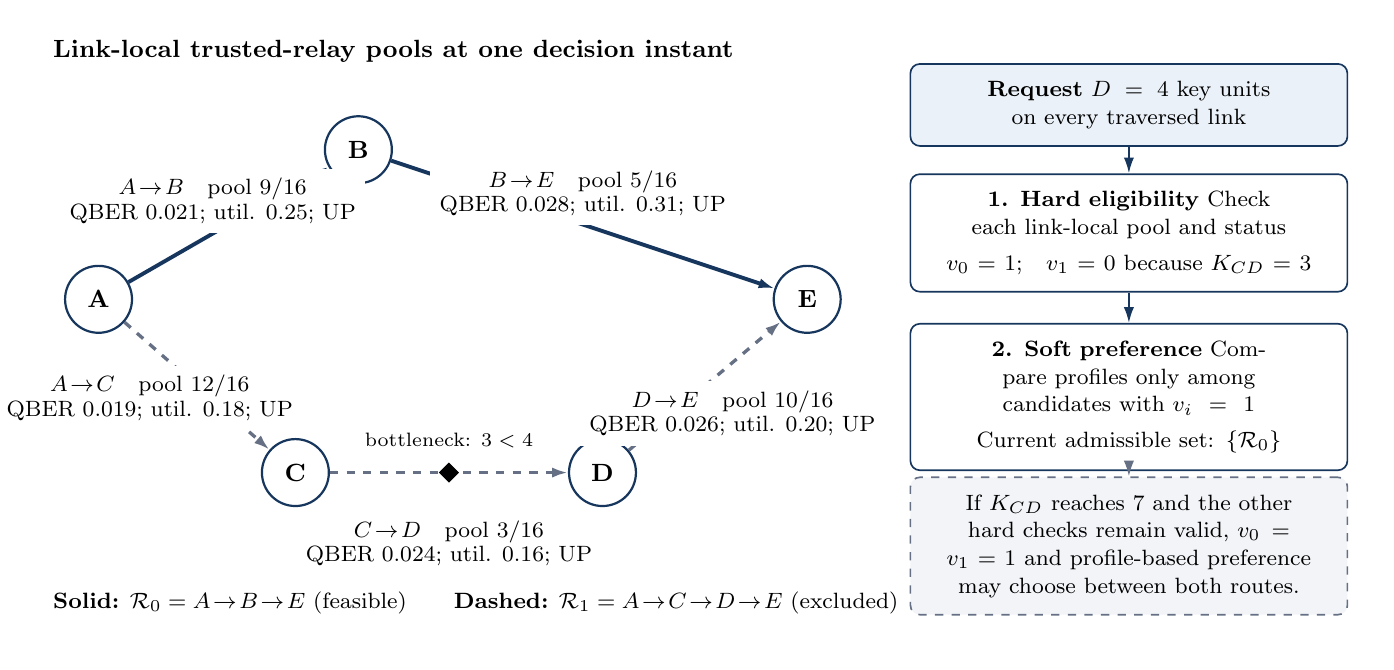
\begin{tikzpicture}[x=1cm,y=1cm]
  \path[use as bounding box] (-0.2,-4.25) rectangle (16.8,3.55);

  \node[qlabel,anchor=west,font=\fontsize{9}{10.5}\selectfont\bfseries]
    at (0,3.25) {Link-local trusted-relay pools at one decision instant};

  \tikzset{
    site/.style={circle,draw=QFlowNavy,fill=white,minimum size=8.5mm,
      line width=0.8pt,font=\fontsize{9}{10}\selectfont\bfseries},
    feasible/.style={qarrow,line width=1.4pt},
    excluded/.style={-{Latex[length=2mm,width=1.3mm]},line width=1.2pt,
      dashed,QFlowGray},
    edgeinfo/.style={font=\fontsize{7.7}{8.8}\selectfont,align=center,
      fill=white,inner sep=1.2mm}
  }

  \node[site] (A) at (0.7,0.1) {A};
  \node[site] (B) at (4.0,2.0) {B};
  \node[site] (C) at (3.2,-2.1) {C};
  \node[site] (D) at (7.1,-2.1) {D};
  \node[site] (E) at (9.7,0.1) {E};

  \draw[feasible] (A) -- (B);
  \draw[feasible] (B) -- (E);
  \draw[excluded] (A) -- (C);
  \draw[excluded] (C) -- (D);
  \draw[excluded] (D) -- (E);

  \node[edgeinfo] at (2.15,1.35) {$A\!\rightarrow\!B$\quad pool $9/16$\\QBER 0.021; util. 0.25; UP};
  \node[edgeinfo] at (6.85,1.45) {$B\!\rightarrow\!E$\quad pool $5/16$\\QBER 0.028; util. 0.31; UP};
  \node[edgeinfo] at (1.35,-1.15) {$A\!\rightarrow\!C$\quad pool $12/16$\\QBER 0.019; util. 0.18; UP};
  \node[edgeinfo] at (5.15,-3.00) {$C\!\rightarrow\!D$\quad pool $3/16$\\QBER 0.024; util. 0.16; UP};
  \node[edgeinfo] at (8.75,-1.35) {$D\!\rightarrow\!E$\quad pool $10/16$\\QBER 0.026; util. 0.20; UP};

  \node[diamond,draw=black,fill=black,minimum size=2.4mm,inner sep=0pt]
    (bneck) at (5.15,-2.1) {};
  \node[qsmall,anchor=south,fill=white,inner sep=0.8mm] at (5.15,-1.87)
    {bottleneck: $3<4$};

  \node[qlabel,anchor=west] at (0,-3.75)
    {\textbf{Solid:} $\mathcal R_0=A\!\rightarrow\!B\!\rightarrow\!E$ (feasible)\qquad
     \textbf{Dashed:} $\mathcal R_1=A\!\rightarrow\!C\!\rightarrow\!D\!\rightarrow\!E$ (excluded)};

  \node[qsoft,minimum width=5.55cm,text width=4.95cm,anchor=north west]
    (request) at (11.0,3.1) {\textbf{Request}\ $D=4$ key units on every traversed link};
  \node[qbox,minimum width=5.55cm,text width=4.95cm,anchor=north west]
    (hard) at (11.0,1.7) {\textbf{1. Hard eligibility}\ Check each link-local pool and status\\[1mm]
    $v_0=1$;\quad $v_1=0$ because $K_{CD}=3$};
  \node[qbox,minimum width=5.55cm,text width=4.95cm,anchor=north west]
    (soft) at (11.0,-0.20) {\textbf{2. Soft preference}\ Compare profiles only among candidates with $v_i=1$\\[1mm]
    Current admissible set: $\{\mathcal R_0\}$};
  \node[qoutside,minimum width=5.55cm,text width=4.95cm,anchor=north west]
    (later) at (11.0,-2.15) {If $K_{CD}$ reaches 7 and the other hard checks remain valid, $v_0=v_1=1$ and profile-based preference may choose between both routes.};
  \draw[qarrow] (request) -- (hard);
  \draw[qarrow] (hard) -- (soft);
  \draw[qdasharrow] (soft) -- (later);
\end{tikzpicture}
\end{document}
